\documentclass[11pt]{article}

\usepackage{amssymb,amsmath,amsfonts,eurosym,geometry,ulem,graphicx,caption,color,setspace,sectsty,comment,footmisc,caption,natbib,pdflscape,subfigure,array,hyperref,epigraph,multirow}

\normalem

\onehalfspacing
\setlength{\parskip}{0.1em}

\newtheorem{theorem}{Theorem}
\newtheorem{corollary}[theorem]{Corollary}
\newtheorem{proposition}{Proposition}
\newenvironment{proof}[1][Proof]{\noindent\textbf{#1.} }{\ \rule{0.5em}{0.5em}}

\newtheorem{hyp}{Hypothesis}
\newtheorem{subhyp}{Hypothesis}[hyp]
\renewcommand{\thesubhyp}{\thehyp\alph{subhyp}}

\newcommand{\red}[1]{{\color{red} #1}}
\newcommand{\blue}[1]{{\color{blue} #1}}

\newcolumntype{L}[1]{>{\raggedright\let\newline\\arraybackslash\hspace{0pt}}m{#1}}
\newcolumntype{C}[1]{>{\centering\let\newline\\arraybackslash\hspace{0pt}}m{#1}}
\newcolumntype{R}[1]{>{\raggedleft\let\newline\\arraybackslash\hspace{0pt}}m{#1}}

\geometry{left=1.0in,right=1.0in,top=1.0in,bottom=1.0in}

\begin{document}

\begin{titlepage}
\title{The Complex Economics of Artificial Intelligence}
\author{Juan Mateos-Garc\'{i}a\thanks{Nesta, 58 Victoria Embankment, EC4Y 0DS, London, United Kingdom. E-mail: juan.mateos-garcia@nesta.org.uk}}
\date{\today}
\maketitle
\begin{abstract}
\noindent TO BE WRITTEN
\bigskip
\end{abstract}

\setcounter{page}{0}
\thispagestyle{empty}
\end{titlepage}

\section{Introduction}
The Law of Requisite Variety states that an organization needs to be as complex as the system it seeks to control: those that operate in fast-changing, dynamic environments need to be flexible, adaptable and able to improvise in response to new situations. Humans have these qualities, and this is why they still play such an important role in creative, innovative organizations. But complexity can be hard and expensive to manage. It requires coordination and the exercise of attention, an scarce resource in information-rich environments. This is why, very often, organizations seek to simplify their internal and external environment through routines and processes (such as the standard forms through which bureaucracies classify many different possibilities into a small number of cases), or use markets to tap into external sources of complexity. 

Today, Artificial Intelligence (AI) technologies are increasingly allowing organizations to respond more flexibly to complex situations. Once trained on labelled data or simulated scenarios, they are able to mimic (to some extent) the flexibility of humans at a low cost and in more predictable ways (some times). They can also help remove biases in human decision-making (these biases are another strategy through which human simplify their environment), and help control in real-time complex systems generating vast streams of unstructured data, such as digital and energy infrastructures, or internet platforms with billions of users. AI's potential applications are pervasive and increasingly necessary in economies that become more complex as they develop. This is why it is being recognized as the latest example of a General Purpose Technology (GPT) that has the potential to transform many different industries, bringing with it a new `techno-economic paradigm'. 

Perhaps unsurprisingly, the introduction of AI across the economy brings with it an increase in its complexity. This is visible in the need for change: New skills are needed and others become obsolete. New business models, organizational practices and infrastructures need to be developed, but there is uncertainty about what these are, or how to coordinate their supply. Markets also become more complex. Transactions that used to be predictable (because they were based on standard parameters, such as a single price) become fluid, and decisions that used to be explainable (because they were undertaken by humans) become opaque. New types of failure emerge.  AIs are after all imperfect - in particular, they remain much more narrow and brittle than the human intelligences they try to emulate- and therefore prone to breaking in unexpected ways, to dumbly optimize the wrong goals, and to be manipulated by opportunist and malicious users, or to engage in emergent behaviours when they interact with each other in the wild. AI also creates complex dynamics between different groups who may prefer others to bear the brunt of AI disruption and uncertainty, potentially bringing with it injustice ans social unrest. As AIs and all their complementary infrastructures are deployed, they create trajectories of technological and economical development that build their own momentum and be hard to shift further down the line. All this increases the complexity that human societies need to be able to understand (through research) and manage (through policy) in order to achieve their goals. These are some of the issues I explore in this essay.  

The essay draws on a growing body of research on the Economics of AI, and particularly on the papers presented in the NBER Economics of AI workshops organized in Toronto in 2017 and 2018. I make an explicit attempt to explore some of the interconnections between issues that have been considered separately until now and which may have to be addressed through collaborations between disciplines, innovations in research methods and data sources, and in policy institutions and processes. As I do this, I tap into key concepts from the Science, Technology and Innovation studies literature that are useful for understanding General Purpose, path-dependent technologies and the systems through which they are developed and adopted, and key references from the AI and ML research related to their economic potential, and some of their limitations. 

\subsection{Structure}
\ref{subsec:structure}

 I begin in Section \ref{sec:definition} by defining AI as \textit{assembles of machine learning predictors that augments and automate decision-making}, replicating commonplace human capabilities such as seeing, hearing and moving, alleviating human biases, and parsing datasets too large and complex for human decision-makers. AI is economically valuable because it takes an abundant input (data) and transforms it into valuable decisions. I present evidence suggesting that AI is a General Purpose Technology (GPT) that could impact productivity, innovation and employment across the economy. The direction of its impact on jobs - and area of great policy and research interest - is uncertain given AI's tendency to displace (eliminate) some jobs, augment others, and create new industries. AI also has important limitations which raise questions about its actual (as compared to potential) applicability in different domains. AI systems are after all highly specialized (narrow), their performance degrades when the environment changes (brittle) and these changes in performance are difficult to predict because advanced AI systems are poorly understood (opaque). This creates uncertainty about the net benefits of AI in different situations and how they will be distributed, and the investments in complementary resources and capabilities such as data, skills, business process and infrastructures that are required to enhance these benefits and enhance their fairness. This uncertainty might lead to market and system failures in AI deployment which I explore in the rest of the essay.
 
 In section \ref{sec:micro} I consider the dynamics of development and adoption in AI ecosystems of AI algorithms, researchers, adopters, individuals and societal actors. I argue that uncertainty about the impact of AI and the distribution of its benefits could create a thicket of informational market failures between these actors. Researchers developing new R\&D technologies may have incentives to exaggerate their potential benefits, downplay their risks, focus their activities on dangerous dual-use applications, or make their research hard to reproduce to hinder competitors. Adopters may deploy AI in ways that are unsafe, generate negative externalities or exploit users. Misaligned AI agents may over-fit, optimize goals that diverge from their adopters or wider society, and be gamed or generate `algorithmic crashes' when they are deployed in complex situations. Without government intervention, this thicket may result in races to the bottom where AI is adopted carelessly and unsafely, abandonment of AI in the face of uncertainty and mistrust about its deployment, or AI internalization if organizations in-house AI to reduce transaction costs and hold-up by others, further intensifying the tendency towards market concentration we see in data-rich markets. 
 
 In section \ref{sec:macro} I focus on social coordination and political economy issues. I present the decisions to adopt AI as games between individuals who have dual economic roles as consumers and workers. Myopic, self-seeking individuals may prefer mild or no adoption of AI in their industry, and strong, potentially labour displacing adoption in other industries (if this brings larger reductions in prices or more convenience in services). Without coordination, their decisions could create excessive levels of job displacement, specially if the future costs of data-powered monopolies, degraded working conditions or mass unemployment are heavily discounted. Further, powerful actors may be able to hinder the adoption of AI in their industries and incentivize their strong adoption elsewhere. Actors who derive their income from capital may have incentives to encourage strong adoption of AI everywhere. All this could increase inequality and social conflict.
  
 In section \ref{sec:irreversibilities} I focus on the dynamic aspects of AI deployment using the concept of path dependence: this is the notion that once a technology is deployed, a business model is socially accepted, and certain social groups gain dominance (while others lose power), the resulting system could be difficult or impossible to modify even if it is found to be worse than alternative paths of development. I contend that today we are at a stage in AI's trajectory where there is still flexibility about the way forward, but this might not last. An implicit recognition of this dynamic is informing the current `AI global race', as different interests pursue the deployment of AI paradigms strongly aligned with their goals and values. 






 Section \ref{sec:onclusion} concludes with some research and policy implications from all the above. On the normative side, I highlight key ethical issues such as fairness in AI impacts, accountability for AI-enabled decisions and agency in human action as AI systems become more influential in economic and social processes. I note that the ability to exercise agency may be irreversibly altered or degraded by the adoption of AI, potentially undermining the foundations for free-markets and liberal democracy. If this is to be avoided, it may be necessary to encourage the development of AI technologies that are agency-augmenting rather than agency-displacing.
 
  On the research side, I call for a new `Social Science of the Artificial' that integrates multiple disciplines and perspectives with the goal of removing current uncertainties about the impacts of AI and the complementary investments required to ensure that AI develops in societally beneficial directions, and identifying effective strategies to encourage development in those directions. On the policy-side, I outline some elements of a policy programme to make the development and adoption of AI more transparent, inclusive and competitive, and to maintain technological and economic diversity in the AI landscape in order to avoid premature lock-in to irreversible, undesirable AI trajectories. This will require an explicit elucidation of human and social goals and values, a mirror of the Turing test where human societies learn about themselves through their responses to the opportunities and challenges emerging from the development of powerful AI technologies. 



\section{Definitions and impacts}
\label{sec:definition}

This section focuses on the economic functions of AI. I begin by defining AI and considering its role within organizations and industries. This analysis highlights the general purpose of AI, which I discuss together with its potential impact on jobs. I then describe features of current implementations of AI which may limit its applicability and/or create risks when it is misapplied, and consider what this means for the rest of the essay.

\subsection{AI definitions, ecosystems and inputs}
\label{subsec:systems}
Economic decisions allocate scarce resources between alternative ends. They create benefits but also have costs because they require the employment and organization of agents that, when faced with information about an economic situation, make a decision\footnote{This includes the costs of contracting with the agent and monitoring her behaviour in situations of imperfect information.}. Organizations economize on these costs by creating routines and processes that respond to the environment with specific actions, but the range of their repertoire has been traditionally limited\footnote{This means that they tend to ignore the unique features of a new situation, or only consider a subset of relevant features them. This means that the fit between action and situation is likely to be poor, and the outcomes inferior to what can be obtained with a more responsive system.}. AI is a `smarter' kind of routine that learns from an abundant supply of historical, digitized data appropriate responses to the environment . It increases the number of intelligent (i.e. context-specific) decisions that an organization can make economically, enabling personalization and interactivity in its products and services and providing the foundation for a `mass decision' economy.

More specifically, Artificial Intelligence (AI) is an \textit{assembly of machine learning predictors that augments and automate decision-making}. Machine Learning (ML) algorithms extract patterns (models) from training data (\textit{supervised machine learning}), or learn effective strategies through trial and error (\textit{reinforcement learning}). The models thus learned can be used to generate predictions about new observations. These predictions (statements about possible states of the world given existing data) enter reward functions that also take into account the benefits and costs of different scenarios to inform or automate decisions. These reward functions can be completely embedded into an AI, which then makes decisions automatically (as is the case with a self-driving car or an AI targeted advert), or involve humans who combine the AI prediction with their judgment about the best course of action to make a decision (think of a radiologist who combines the AI analysis of a patient scan with her expert knowledge to recommend a treatment).

The difference between AI and ML is subtle: AI is a practical application of ML algorithms, often combining several of them that generate a range or sequence of predictions which are integrated to inform decisions. An example of this would be an anthropomorphic robot that uses computer vision, simultaneous localization and mapping and motion control to navigate an environment. It is also useful to think of AI in terms of degree. We say that a decision system has a higher degree of Artificial Intelligence when it requires less human involvement at key stages - that is, when the predictions that it generates are a stronger determinant of subsequent decisions and actions. An automated decision-making is more AI than a merely advisory one (although that will not make the decisions that it makes more intelligent).

AI takes the following inputs: 

\begin{itemize}
    \item \textbf{Training data} with examples that the AI can learn from. This can be internal data, a publicly available benchmark dataset or synthetic data generated through simulations or Generative Adversarial Networks optimized to generate realistic data.
    \item \textbf{Computational resources} used to store and process the data and execute the search, optimization and simulation processes through which AIs learn from it.
    \item \textbf{Software} implementing AI algorithms. This software can be developed in-house, licensed from external sources, or modified from open source implementations. 
    \item \textbf{Analytical human labour and capabilities} to design and implement the technologies underpinning AI. This might involve making decisions about what data and variables in the data (`features') and models to use or what parameters to select during optimization.
    \item \textbf{Supervisory human labour and capabilities} that use judgment (evaluation of options under uncertainty) to define or apply reward functions, and identify errors in the predictions and recommendations from AI.
    \item \textbf{Implementer human labour and capabilities} that execute decisions informed by AI, such as when a doctor gives a patient a recommended treatment, or a worker in a warehouse dispatches a sale generated by an AI targeted ad.
\end{itemize}

These decision-making processes have a hierarchy of goals: An AI searches the model, parameter and feature space for configurations that generate predictions with optimum accuracy, minimum prediction error or maximizing rewards. Effective reward functions are (or should be) designed to lead to actions maximizing the net present benefit of a decision for the organization. These actions are executed using other processes and skills, and ultimately contribute to achieve operational and strategic goals that advance the agenda of the organization. These actions are part of wider social systems of decision-making such as markets, industries or public sectors: they interact with the actions of other agents such as competitors and consumers that have their own decision-making processes, and collectively create outcomes that generate feedback and new data, and can modify demand for inputs (for example, if AI systems develop capabilities that augment or displace human labour previously involved in certain types of decisions). 

Consider for example a social media platform such as Facebook: it is powered by AIs that recommend information and connections to its users, tags content with relevant labels (e.g. people's faces) and identifies inappropriate content. These AIs are trained to maximize user engagement and interaction, and to minimize errors when making predictions. These actions increase the number of users in the platform an the amount of time that they spend there, attracting advertisers to the platform and increasing Facebook's profits. However, some of these users might want to use the platform to distribute spam, or violent or inflammatory content. They will behave strategically to game its AIs and spread that information. Also, high engagement with Facebook may be detrimental for users' health and its reputation and long-term sustainability. All these considerations highlight the complex interactions between different types of goals in AI systems, and the risk of coordination failures and breakdowns in the system when goals are not aligned or actors behave strategically. I focus on these questions in \ref{sec:micro}.

Figure \ref{fig:ecosystem} represents this AI ecosystem.

\begin{figure}
    \centering
    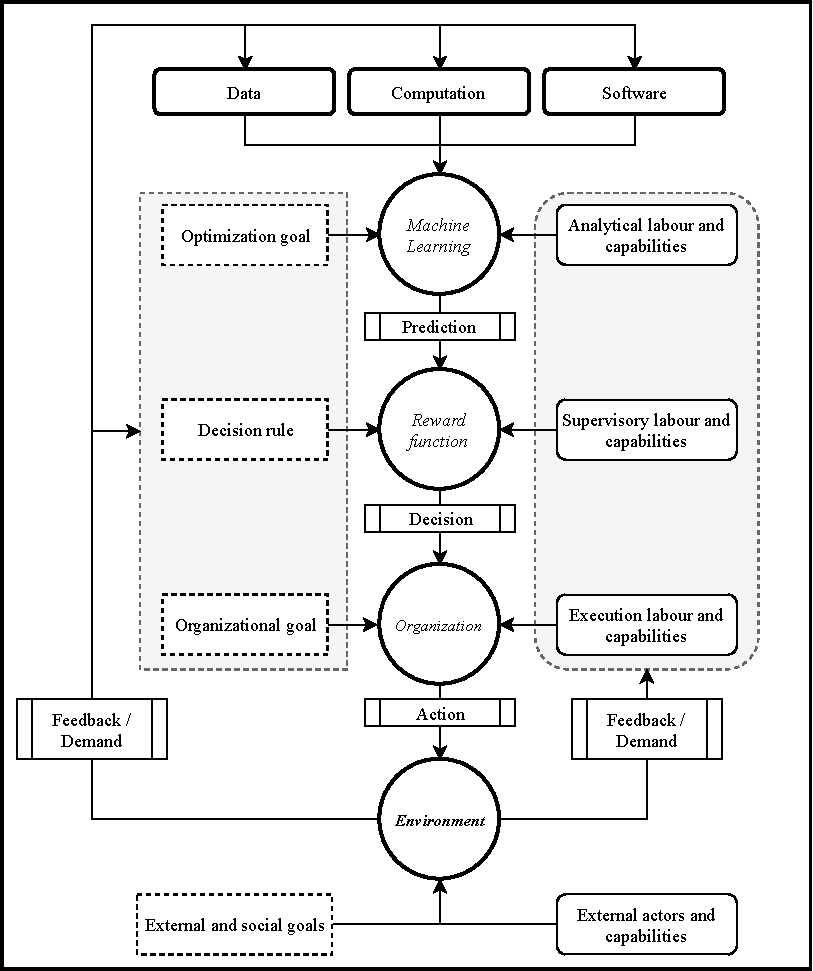
\includegraphics{ai_diagram.pdf}
    \caption{\textbf{The AI ecosystem:} This diagram represents the flow of information and other inputs and outputs in an AI ecosystem.}
    \label{fig:ecosystem}
\end{figure}

\subsection{Generality}
\label{subsec:general}
Recent advances in AI have been driven by a mix of supply push and demand pull factors. 

\begin{itemize}
    \item On the \textit{supply push side}, there has been a rapid increase in the quantity and quality of key inputs for AI: more labelled data from internet sources, cheaper computation and storage from better hardware and cloud computing, and innovations in ML algorithms, particularly with the development of powerful artificial neural networks that extract abstract patterns (features) from unstructured data such as images, video or sound with less need from human intervention (\textit{deep learning}), and reinforcement learning systems that automatically adapt their strategies to feedback from the environment in order to optimize their performance. 
    \item On the \textit{Demand pull side}, the digitization of organizations and markets has created `big data' (large volume, variety and velocity) datasets that cannot be economically analyzed by human researchers, and require automation in analysis. The popularity of online platforms for search, e-commerce and match-making has created demand for systems able to filter and recommend relevant information and content, and personalize services. The increasing complexity of technical systems and infrastructures demand real-time control and optimization integrating a large volume of interacting factors which human monitors with limited processing capability cannot parse effectively.
\end{itemize}

Together, these factors have resulted in rapid improvements in AI and their practical application in domains such as computer vision, natural language processing, speech synthesis, mobility and game playing, and to the creation of digital systems that make large volumes of automated decisions based on these capabilities. Some examples include recommendation engines for retrieving and targeting information, images and video, classification systems that label images with comparable accuracy to human experts, natural language translation and recognition systems, and autonomous vehicles and robots that can operate in less controlled environments, and with less need for human supervision than before. In addition to imitating commonplace human skills at scale, AI systems can also go beyond human capabilities, thus augmenting human decision-making. For example, AI are, at least in theory, less prone to cognitive biases than humans, so they can complement and enhance human decisions in domains such as recruitment, finance or the law\footnote{This assumes unbiased input data and a stable decision environment. I focus on the problems that emerge when these conditions are not fulfilled next sub-section.}. AI can also extract information from big, fast data-sets obtained from multiple streams to control and optimize complex systems such as energy infrastructures.

The breadth of areas where AI is being and/or could conceivably be applied strongly suggest that it has the characteristics of a General Purpose Technology (GPT): this means that it is technologically dynamic (susceptible to rapid improvements in performance), applicable in many industries, and able to generate follow-on innovations in these new application areas. Recent analyses of the development and diffusion of AI in different academic disciplines, computer science domains and industries are consistent with this idea. The levels of R\&D activity related to AI has increased, AI topics are appearing in other sectors and disciplines, and they are proving influential wherever they do (Figure \ref{fig:dl} illustrates this trend in a corpus of Computer Science pre-prints from \texttt{arXiv}, a repository widely used by AI researchers and engineers). 

\begin{figure}
    \centering
    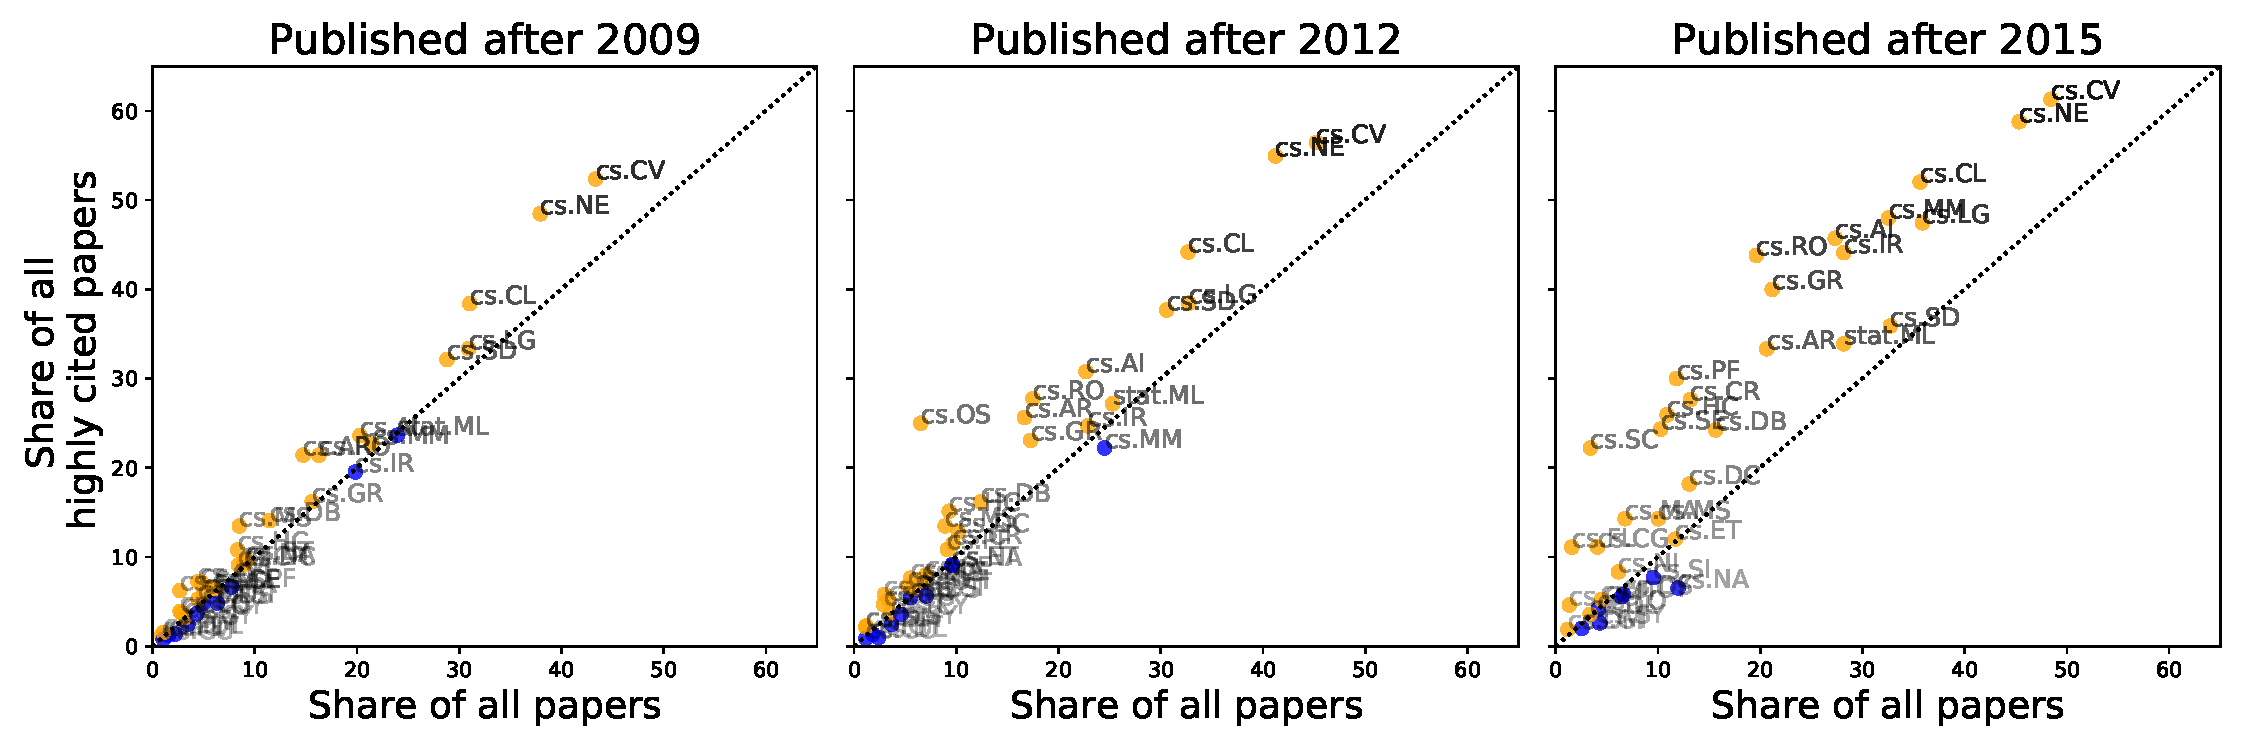
\includegraphics[width=\textwidth]{figure_2.pdf}
    \caption \textbf{Deep Learning (DL) papers as a share of all papers by computer science category in the \texttt{arXiv} preprints website, and as a share of all highly cited papers in that same category}. Left panel shows all papers published after 2009, Centre panel shows all papers published after 2012, and Right panel shows all papers published after 2015. The figure shows that, in more recent vintages of papers, DL represents a larger share of papers in a category (a general displacement of fields towards the right) and a larger share of influential papers a general displacement of papers upwards. This is consistent with the idea that DL is becoming more important and influential in a growing number of computer science fields.
    \textbf{Source}
    \label{fig:dl}
\end{figure}

Ultimately, AI could greatly improve productivity by making the delivery of existing products and services more efficient, and creating new industries based on automated decision-making. Further, AI is an `invention in the methods of invention' that could improve the productivity of scientific discovery and invention processes by, for example, enabling a faster and more comprehensive exploration of opportunities in research fields such as pharmaceutics or material science where innovations involve combinations of components within a vast search spaces which can now be explored more comprehensively by AI agents. This way, AI could countervail stagnating productivity in science and technology (the fact that `good ideas are getting harder to find') and drive productivity and economic growth in years to come.  The potential applications of AI are of course not limited to the private sector. Recent policy documents suggest that AI could be pivotal in tackling important social challenges from an aging population to environmental sustainability. 

The deployment of a GPT requires complementary investments across the economy: this includes the development of new skills, processes and technical and social infrastructures, as well as innovations in the way in which production is organized, and in business models. It is often said that the impacts of the electricity GPT in industrial productivity did not materialize until factories radically reorganized their layout to reap the benefits of flexible electric motors, decades after its arrival. AI may require similar innovations in organization and processes, involving business experiments and coordination between multiple agents, including developers of AI technologies and their adopters across the economy, as well as the suppliers of complementary resources such as skills and infrastructures. Uncertainty about which are the most effective combinations of technologies and capabilities, and externalities between different agents (for example if organizations decide to `wait and see' until there is better knowledge about the most suitable models to adopt AI, or if the benefits from experiments in one sector spill into another) could lead to under-investment in AI, slow down its deployment and dampen its benefits. In Section \ref{sec:micro} I outline some of the coordination challenges raised by this. For now, I will simply note that those industries where the key inputs for AI development are more readily available will develop it faster, and reap its benefits sooner. Later sections \ref{subsec:irreversible} considers potential externalities from unevenness in AI development.

\subsection{AI, jobs and inequality}
\label{subsec:jobs}
One economic dimension of AI that has received particular attention is its impact on jobs: as previously mentioned, there are many domains where state-of-the-art AIs are reaching human-level of capability,  suggesting that they could be used to replace human workers in relevant industries. Several studies have estimated the share of the workforce `at risk of automation' based on the current task composition of different occupations, the capabilities required to undertake those tasks, and the extent to which those capabilities could be replaced by AI. Here it is assumed that routine physical and cognitive capabilities will be easier to automate, while non-routine cognitive (creative) tasks and tasks involving social skills will remain the preserve of human workers. 

These studies assume that human jobs and skills will not change, that organizations have incentives to adopt AIs which also have important limitations (I discuss these below), that it will be possible to replace flexible human decision-makers with `narrow' AIs whose repertoire of tasks is limited, and that there will be no policy interventions or regulations to limit the automation in jobs in certain domains for legal or cultural reasons. 

They also neglect to consider that the adoption of AI in a sector does not only displace jobs (\textit{labour displacement}). It can also bring gains in productivity which increase demand for its products, and for labour working in complementary roles (as happened with bank tellers after the introduction of Automated Teller Machines in the 1970s) (\textit{labour augmentation}), and lead to completely new types of industries, jobs or tasks such as those involved in the design, development and monitoring of AI reward functions (\textit{new labour catalysis}). Several empirical studies have sought to estimate these impact in those industries and locations more strongly exposed to industrial robots, showing that robotization has improved industrial productivity but also displaced jobs. One important point made in this literature is that one can imagine scenarios where businesses adopt `mediocre' AIs that displace workers while only making modest contributions to productivity, or AIs which increase the supply of labour in other sectors, depressing wages and reducing the incentives to invest in productivity-enhancing technologies. Some of these externalities, which highlight the complex, interrelated nature of the impact of AI on labour markets and prevailing uncertainty about their nature, are discussed in \ref{sec:micro}.

I conclude this brief overview of the growing literature about the impact of AI on labour markets by noting that the deployment of AI  is likely to bring with it an increase in economic inequality, particularly if it displaces workers. The reason for this is simple: AI is a form of capital. As it is increasingly deployed, the share of capital in economic output increases. Since capital ownership and income from capital tend to be more concentrated than income from labour, this should increase the share of output going to the owners of capital, and economic inequality. An interesting aspect of this situation which I focus on in Section \ref{subsec:macro} is that capital owners who experience benefits from the deployment of AI without any of the costs in terms of displacement and disruption, may have incentives to encourage its deployment at levels which are detrimental for other social groups, and that further increase inequality.

\subsection{AI Limitations and risks}
\label{subsec:limits}
I just mentioned that current implementations of AI are  `narrow'. How could this be, if AI is a General Purpose Technology? The reason is that even though AI is a collection of technologies and methods that can be applied to inform a vast range of decisions in many industries - it has many different use cases - once an AI is implemented to address a particular use-case, its generality becomes greatly restricted. AI narrowness has several dimensions:

\begin{enumerate}
    \item AIs are highly specialized, inefficient learners: In order to inform decisions in a domain, they need to be trained with large amounts of data from that domain. The learning they acquire is highly specific to that context, and difficult or impossible to transfer to new areas.
    \item AIs are greedy learners: they maximize the amount of information that is extracted from the training data, but this creates the risk that they `over-fit' (learn noise in the training set) and lose the ability to generalize to new information\footnote{ML researchers use methods such as \textit{regularization} (penalizing excessively complex models) and \textit{cross-validation} (evaluating models in test data-sets they were not originally trained on) to reduce overfit, and make their models more generalizable and robust}. This also makes AIs undiscriminating: they will extract information from the data regardless of its quality. AIs trained on biased data will incorporate those biases into their model of the world (this is a manifestation of the \textit{Garbage In, Garbage Out} principle). This can be a particularly concern if AI is applied in domains where existing datasets reflect social injustice or prejudices, as may be the case with the criminal justice system, university admissions or access to credit.\footnote{For example, if ethnic minorities are more likely to be arrested, or if they are more likely to re-offend due to discrimination in the labour market or policing, this will create a skewed dataset. Model prediction will reflect these biases, rather than some ground truth about, say, criminal propensities among different social groups.}  
    \item AIs are brittle learners: Related to the point above, AI performance degrades if it is exposed to inputs that were not present in the training data. However, unexpected and rare situations are likely to occur in real-life environments, the environment may change, or actors in those environments may seek to manipulate AI systems, resulting in AI errors and failures\footnote{A salient case of this are \textit{adversarial examples} that create catastrophic declines in performance when inputted into an AI system.}.
    \item AIs are mindless learners: They literally optimize a pre-set performance metric or reward function even if this generates unexpected side-effects or creates situations that contradict the goals of their organization. This means that the goals of AI systems have to be carefully aligned with those of the organization deploying them in order to avoid surprising and unsafe AI behaviours.
    \item AIs are opaque learners: The optimization procedures that AIs follow in order to learn from data can be hard to interpret and explain. This makes it hard to predict their behaviour (e.g. their failure modes) and to explain their outputs, rendering them unaccountable. Current theoretical understandings of the operation of state-of-the-art AI systems based on deep learning are still imperfect.\footnote{This mirrors the situation in the early days of the Industrial Revolution, where practical ($\Omega$) knowledge (know-how) about how to apply the steam engine raced ahead of theoretical ($\Lambda$) knowledge (know-why) about the physical processes underpinning its performance.}.
\end{enumerate}

AI's narrowness contrast with the flexibility of human decision-makers equipped with common sense which allows them to improvise when faced with new situations, a causal understanding of the relationship between different variables enabling more robust predictions about future scenarios and the behaviours of others, and background knowledge of social and organizational values within which their predictions and decisions are embedded. Several streams of AI research seek to address these limitations of AI systems, increasing their flexibility, robustness, alignment and transparency.

\subsection{Implications}
\label{subsec:implications}
AI stands to transform productivity and innovation across the economy by enabling more, better and new decisions in many different industries. Realizing these benefits requires new combination of AI technologies with complementary factors and capabilities, but there is uncertainty about what are the most suitable combinations, and their impacts (including on jobs). The limitations in state-of-the-art AI systems which I just reviewed suggest that there are also risks in its deployment, potentially resulting in algorithmic errors, catastrophic failures, or the optimization of undesirable goals: a penalty coefficient needs to be applied when AIs are applied to a new use-case, and their contribution to output degrades over time following a depreciation coefficient with a schedule tracking (unpredictable) changes in the environment. The value of these coefficient is unknown, as are their interactions with the aforementioned complementary inputs, as well as the behaviours of other agents.

For the rest of the essay, I focus on potential market failures stemming from this complexity: In Section \ref{sec:micro} I focus on issues around development and adoption of AI, Section \ref{subsec:macro} considers political economy and social dilemmas, and Section \ref{subsec:irreversible} discusses the path dependent nature and potential irreversibilities of AI innovations and investments being undertaken today. Section \ref{subsec:conclusion} sets out a research agenda to avoid these risks and realize the economic and social potential of powerful AIs.

\section{Market and system failure in AI ecosystems}
\label{sec:micro}
Here I show that uncertainty about the impacts of AI and its complements, misalignment in incentives between the agents involved in the AI ecosystem, and information asymmetries between them, create a tangle of potential market failures in AI development and adoption \footnote{I use the term `market failure' broadly to include all situations where misalignment in incentives between different actors create deviations from an ideal situation in the development of AI.}. After introducing these actors, their activities and their goals, I present an ideal configuration of the ecosystem for AI development and adoption with perfect information, deviations from this ideal, and potential outcomes.

\subsection{Actors in the AI development and adoption ecosystem}
The AI ecosystem in Figure \ref{fig:ecosystem} involves a group of actors that undertake important activities in the development and adoption of AI. Together, they determine its trajectory and outcomes .

\begin{itemize}
    \item \textbf{AI agents} are the algorithms themselves. Although I obviously do not assume that these AI agents have `agency' or consciousness, they nevertheless have direct goals (metrics and rewards functions to optimize) and indirect goals (the goals of the organization implementing them, to which the achievement of the indirect goals should contribute).
    \item \textbf{Researchers} are the scientists, researchers and engineers who develop and apply ML algorithms and AIs, working both inside adopter organizations and in public research organizations and universities. I assume that these individuals seek to advance the state of knowledge in AI research and the performance of AI, to gain acclaim among their peers, and to access research funding.
    \item \textbf{Adopters} are organizations that deploy AI to achieve their organizational goals - for example, to increase profitability, reduce costs or improve effectiveness in the delivery of a public service.
    \item \textbf{Individuals} include users, consumers and workers participating in AI ecosystems: they create data that is used by AI, interact with AI-derived predictions and decisions, and work in environments where AI has been or might be adopted for a variety of purposes, such as optimizing productivity or monitoring worker efforts. Individuals have multiple, perhaps conflicting goals such as maintaining and improving their personal and political rights, working conditions and salaries, and accessing affordable and convenient goods and services.
    \item \textbf{Society} refers to the polity within which the AI system is embedded. It funds public goods and uses a variety of instruments to encourage societally beneficial behaviours and discourage societally detrimental behaviours. We assume (idealistically) that this society is well-ordered, and that its goal is the well-being and prosperity of its citizens and harmony between its constituent communities. It is represented in the AI ecosystem by public agencies such as research funders or regulators. 
\end{itemize}

\subsection{Ideal scenario}
We can, as a benchmark, imagine an ideal situation with perfect information where the AI ecosystem for the development and adoption of AI performs efficiently: 

-Researchers develop AI algorithms using reproducible methods that others can review and assess, taking into account social and business needs and clearly communicating the strengths and limitations of the technologies they develop. 

-AIs are themselves transparent and well understood, easy to implement in a way that is aligned with organizational goals, and unlikely to generate unexpected effects (or at least the types of algorithms and contexts where such effects are likely to occur are well understood, so that risks can be managed). 

-Adopters select those algorithms with the greater value for them and implement them transparently and safely, together with suitable complementary investments. In doing this, they take into account the rights of their workers, as well as any wider impacts that the AI systems they adopt might have, such as for example in labour markets. 

-Users and consumers are aware of how AI algorithms are being used in the organizations they interact or transact with, and the implications that this has for their personal data and the products and services they are being offered.  They are thus able to make informed decisions about what products and services to consume. 

-All of this takes place in a way that is consistent with societal goals and the regulations to uphold them. 

\subsection{Non-Ideal reality}
\label{subsec:non_ideal}
As I started discussing in Subsection \ref{subsec:limits}, several conditions for `ideal' AI development and adoption fail to hold: there is uncertainty about the benefits of AI in different situations and what are the complementary investments that maximize them, AI limitations and failure modes are not well understood, and aligning AI goals with those of the organizations that adopt them is not trivial. Further, there are multiple asymmetries in information between agents in the system: Researchers are better informed about the characteristics of the AI systems they develop, Adopters know more about the how the AIs are implemented, their performance, and the goals they seek to optimize; Individuals have better information about the data they provide and its veracity. These asymmetries, together with misalignment in objectives and incentives create the conditions for transactions and interactions which might be exploitative, abusive, unfair or generate externalities for other actors in the AI ecosystem. 

Table \ref{tab:info_failures} outlines these `dyadic failures', which I have grouped in five categories:

\begin{table}[h!]
    \centering
    \renewcommand{\arraystretch}{1.5} 
    \begin{tabular}[width=\linewidth]{c c c c c}
    \textbf{Principal \textbackslash  Agent} & \textbf{AI agents} & \textbf{Researchers} & \textbf{Adopters} & \textbf{Individuals} \\
    \hline
    \textbf{AI agents} & Gaming & & Mis-application & Gaming \\ 
    \textbf{Researchers} & Over-fit & Irreproducibility & Dual-use & \\
    \textbf{Adopters} & Misalignment & Exaggeration &  & Sabotaging \\
    \textbf{Individuals} & Unsafety & Hidden Automation & Rights-infringement & \\
    \textbf{Society} & Flash crash & Dual-use & Mediocrity & Dilemmas \\
    \hline
\end{tabular}
    \caption{Dyadic information failures in the AI decision-making system: Each cell represents a market failure behaviour between the column agent and the row principal.}
    \label{tab:info_failures}
\end{table}

\subsubsection*{Manipulation and subversion of AI systems}
Narrow and brittle AI systems can be manipulated and subverted by other actors. For example, these actors might want to use an AI service in a way that contravenes its terms of service, access valuable information from a secure AI platform, or degrade its performance for financial or political reasons.  I use the term \textit{Gaming} to refer to situations where an actor manipulates an AI to behave against its implicit goals. For example, the actor might use misleading language to distribute spam or fake news in a social media platform, or implement a cyber-attack using a strategy that resembles a normal pattern of user behaviour. The gaming actor might be an individual or an AI agent such as for example a bot or a Generative Adversarial Network designed to produce synthetic data hard to classify accurately by the AI defender. \textit{Sabotaging} refers to situations where individuals inside an organization (for example its workers) engage in acts that directly damage AIs or degrade their performance. 

\subsubsection*{Risky implementations}
AI safety risks are situations where insufficient information about the real performance and goals of an AI system lead to an implementation with reduced benefits, hidden costs or insufficient safeguards. Here, it is important to note that the organization adopting the AI does not benefit consciously from these risks. Other things being equal, it would prefer to avoid them in order to avoid negative publicity and/or legal consequences. It may however benefit unconsciously if, for example, risky AIs are cheaper to implement than safe ones, or they bring higher average performance at the expense of rare, catastrophic errors or errors confined to minorities within the user-base (e.g. if the AI has been trained on biased data). 

Some risky implementations of AI includes situations where an AI \textit{overfits} the data despite the best efforts of the researcher who designed and developer her. This means that the real predictive performance of the AI agent will be lower than expected when adopted in a real-world scenario, potentially lowering its benefits or creating risks. \textit{Unsafety} refers to interactions between AI agents and consumers or users where the algorithm is liable to make errors detrimental to the individual. A recent example of this is the distribution of unsuitable content to children through the recommendation engine of online video sites. \textit{Misaligned} AI agents pursue goals that diverge from those of the adopter organization. This might be because the AI reward function was insufficiently or imperfectly specified, or the AI was trained on biased data, creating an `omitted payoff bias' (optimizing the wrong metric).  

The final type of AI safety risk is a \textit{Flash Crash} where AIs give rise to unexpected, emergent phenomena such as the flash crash caused by High-Frequency-Trading algorithms in the New York Stock Exchange in May 2010, or political radicalization through the creation of filter bubbles and dissemination of fake news in social media sites. These outcomes are caused by insufficient information about the performance of AIs participating in complex social systems and large platforms involving actors with incentives to game the AI system through novel (out of sample) behaviours, as well as other AIs whose reactions may create oscillations, information cascades and bandwagons.

\subsubsection*{Irresponsible Research and Innovation}
In this case, an actor undertakes AI development and adoption activities that are irresponsible or fraudulent: she does this by exploiting, withholding or neglecting information about the characteristics and impacts of the AI systems that she is developing or adopting because the costs of such behaviours are hidden or incurred by other actors in the transaction or interaction, or in the broader ecosystem. 

One case is \textit{Mis-application}. Here, an AI adopter deploys a narrow AI for an unsuitable task. This could be because it has been trained on data that does not represent its domain, because the stakes are higher than in the original domain it was developed for (the consequences of mistakes are more severe) or because the new domain requires higher levels of interpretability or explainability in outputs. \textit{Exaggeration} refers to situations where researchers overstate the benefits of an AI or understate its costs / risks, potentially leading to its mis-application by adopters, or to an over-supply of funding for research to deliver these benefits. Such behaviour in the AI research community has historically led to `AI winters' with drastic declines in funding for the field after high expectations about its potential impact failed to materialize.

I use the term \textit{Irreproducibility} to refer to a broad range of strategic behaviours by AI researchers which hinder scientific progress in the field. This includes the dissemination of scientific outputs (for example, academic papers describing a new ML algorithm) without the materials required to reproduce it so as to impede competing researchers, or to hide flaws in the work. Also the use of ambiguous language or unnecessary complexity, techniques that over-fit to benchmark datasets, a preference for complex and opaque models with high performance in known metrics over more explainable and transparent approaches whose performance is harder to measure, or a bias towards publishing positive and novel results. All these behaviours create uncertainty about the benefits and costs of new AI methods, and weaken knowledge spillovers between different researchers in the system.

\textit{Dual-use} risks stem from the generality of AI, which creates the possibility that AIs developed for socially beneficial goals (e.g. computer vision systems for self-driving vehicles) might be re-purposed in ethically questionable or dangerous directions (mass surveillance or espionage). This failure may take place between research funders and researchers who carelessly or opportunistically develop risky AIs, or between researchers and malicious adopters. Established norms for research dissemination based on open publications and open source software prevalent in much of AI research hinder the prospects for controlling how and where AI research outputs are applied.  \textit{Hidden automation} is a modality of the dual-use situation where the actions of individual consumers and workers generate data which are, without their knowledge or permission, used by researchers or adopters as training datasets to develop AI systems that automate labour. 

Finally, \textit{Mediocrity} refers to situations where adopters implement AIs with negative impacts on society. In addition to AIs which are misapplied, unsafe or prone to generate flash crashes and unexpected failures, this also includes AIs which degrade the quality of the user experience while saving costs for their adopter, or mediocre AIs that displace labour without inducing productivity gains that could contribute to net increases in employment (this results in an externality for society in terms of increased welfare costs, social unrest etc.)

\subsubsection*{Exploitation}
Situations of exploitation occur when AI is adopted in ways that infringe on the rights of individuals as users, consumers, and workers. This includes applications of AI that infringe on privacy, misuse personal data, attempt to manipulate the behaviours of individuals or encourage them to engage in addictive behaviours, use the data they supply in ways that they would perceive to be unfair (such as for example through price discrimination or discrimination based on protected characteristics such as genre, ethnicity or sexual orientation), as well as applications that put individuals at risk (particularly when they are in positions of vulnerability) or degrade their working conditions. These behaviours are made possible by lack of transparency about whether and how AIs are adopted inside the organization(s) that individuals interact with, and about the benefits that AI generates and how they are distributed.

\subsubsection*{Dilemmas}
To conclude, dilemmas refers to situations where the uncoordinated behaviour of individuals leads to societally sub-optimal AI development and adoption scenarios. I focus on these situations in Section \ref{subsec:macro}.

\subsection{Some outcomes}
\label{subsec:outcomes}
What are the outcomes of the tangle of market failures in AI development and adoption described above? Given the large number of actors involved, and the complex interdependences between their behaviours, one could imagine many different situations depending on the context. Here, I outline two potential `laissez-faire' scenarios (I consider policy interventions in Section \ref{subsec:conclusion}):

First, one could imagine a \textit{race to the bottom} where lack of transparency about the impacts of AI and their distribution result in the careless deployment of AIs for the benefit of adopters through the use of exploitative practices and business models. There are few incentives to invest in measures to make AI safe and ensure the privacy and safety of user data, and those organizations that do are unable to compete with less principled rivals. Unsafe AI technologies display `emergent' behaviours when they spread into high-stake domains and deployed in complex social systems, resulting in flash crashes and systemic failures. Researchers respond to adopter demand developing more powerful but potentially unsafe and unethical AI systems built on a shaky knowledge base due to dubious research practices and a reproducibility crisis. In spite of this, individuals continue using and consuming goods and services based on AI because they are essential, or because they lack information about the way AI are implemented, as well as their impacts and risks.

Another potential outcome is \textit{abandonment}. In this case, individuals stop using AI products and services due to concerns about their implementation and impact, perhaps in response to a catastrophic event or mass AI failure. Funding for AI research is stopped or curtailed, and the use of AIs is restricted to a small number of scenarios where their performance and conditions for effective operation are well understood and regulated. 

A third scenario is \textit{internalization}: the dynamics above increase transaction costs between organizations in AI ecosystems. Organizations are faced with the need to verify and validate any AIs and AI-based goods and services they procure, the risk of hold-up and algorithmic failure due to exploitative and unsafe implementations of AI in suppliers and clients, and the need to reassure consumers against the perception of a race to the bottom in the use of AI. To reduce these transaction costs, they opt for internalizing AI development and adoption, recruiting researchers and acquiring other organizations within the ecosystem. This has the added benefit of restricting competitor access to valuable data / software / analytical skills, and of increasing economies of scale and scope in AI. The resulting concentration in AI activity makes it easier to restrict unsafe and unethical AI applications, but it also creates some challenges, such as a decline/co-opting of public AI knowledge bases and skills potentially raising barriers to AI adoption by other sectors and organizations, and less competitive and more fragile AI ecosystems (concentration of activity in small number of organizations makes them an attractive target for malicious actors, and increases the potential consequences of errors in their AIs and infrastructures).

\section{Social dilemmas in AI deployment}
\label{sec:macro}

Last section focused on the dynamics of AI development and adoption \textit{inside a single sector}. Here, I consider the situation \textit{between sectors}, potentially covering the whole economy. Continuing with the theme of complexity, the main point here is that the deployment of AI is determined by the decisions of multiple agents spread across different sectors and roles. Without coordination between them, there is the risk of social dilemmas leading to extreme levels of AI deployment, and/or strategic manipulations of AI deployment by powerful actors in ways that increase inequality. 

I begin by outlining a simple model with two actors in two sectors, and describe their options and potential payoffs. Then, and as before, I present an ideal scenario where actors coordinate their decisions to reach the societally desirable outcome. I show why this is result is unlikely and why, and conclude with some outcomes. 

\subsection{Set-up}
\label{subsec:setup}
I consider an economy with two sectors, S1 and S2 and two individuals I1 and I2. Each individual selects, through her consumption choices, the level of AI adoption in the other sector (i.e. she chooses goods supplied by firms that have adopted AI at different levels). Each individual experiences employment outcomes and working conditions depending on the consumption choices of the other (i.e. she works - or does not work - in industries that have adopted AI at different levels). Each individual receives a work payoff (salary weighted by working conditions) and a consumption payoff (price weighted by convenience and quality) which depends on joint adoption choices. The AI adoption choices and pay-offs are:

\begin{enumerate}
    \item \textbf{No AI adoption}: In this case, AI is not adopted in a sector. The prices of its products and the working conditions of its workforce remain the same. I assume that this is the baseline, so the worker payoff is 0 and the consumer payoff is 0.
    \item \textbf{Balanced AI adoption}: AI is adopted in a sector in a balanced way. The adopted AI is labour augmenting, thus increasing the productivity of the workforce without worsening working conditions. Prices of the products in the sector decline. Workers in the sector receive a work payoff of 5 due to the increase in productivity, while consumers from the sector receive a consumption payoff of 5 due to decline in prices/increases in convenience and quality.\footnote{Here I am assuming that workers in a sector are not adverse to technological change. In that case, the worker pay-off for balanced AI adoption would be negative, but less so than the worker pay-off in extreme adoption.} 
    \item \textbf{Extreme AI adoption}: AI is adopted in a sector in an extreme way. The adopted AIs are labour displacing so they create unemployment. Those individuals who keep their jobs experience degraded working conditions and lower salaries. Workers in the sector receive a work payoff of -10. Consumers from the sector experience a consumption payoff of 10 due to large declines in prices, improvements in quality and convenience etc.\footnote{As I briefly touched on in Subsection \ref{subsec:jobs}, the increase of productivity in extreme AI adoption sectors may create new economic opportunities for the workers who have been displaced, although this is by no means certain, as I also discussed. In any case, the short-term impact of extreme AI adoption is likely to be highly disruptive for workers in the sector.}
\end{enumerate}

It is important to note that individuals are not considering other impacts brought about by the adoption of AI in a sector, such as for example, declines in safety or increases in market concentration. We assume that these costs are hidden from them due to lack of transparency in AI development and adoption, or are discounted because they will happen in the future. Individuals are also assumed to be selfish: they do not  take into account in their decisions the employment outcomes or working conditions of individuals in other sectors. 

This is all presented in Table \ref{tab:dilemmas}.

\begin{table}[h!]
    \centering
    \renewcommand{\arraystretch}{1.5} 
    \begin{tabular}[width=\linewidth]{c c c c}
    \textbf{Sector 1} \textbackslash \textbf{Sector 2} &  \textbf{No adoption} & \textbf{Balanced adoption} & \textbf{Extreme adoption} \\
    \hline
    \textbf{No adoption} & I1:(0,0) & I1:(0,5) & I1:(0,10) \\ 
    & I2:(0,0) & I2:(5,0) & I2:(-10,0) \\
    \textbf{Balanced adoption} & I1:(5,0) & I1:(5,5) & I1:(5,10) \\ 
    & I2:(0,5) & I2:(5,5) & I2:(-10,5) \\
    \textbf{Extreme adoption} & I1:(-10,0) & I1:(-10,5) & I1:(-10,10)\\ 
    & I2:(0,10) & I2:(5,10) & I2:(-10,10) \\
    \hline
    \end{tabular}
    \caption{Pay-off table in AI adoption: Each individual controls, through her consumption choices, the level of AI adoption in the other sector. The pay-off tuple represents pay-offs for individual working in each sector (I1 and I2). The first value in each tuple represents the work payoff, and the second value represents the consumption pay-off. Although the social optimum is achieved when both individuals select balanced adoption strategies in the other sector, the equilibrium strategies are to select extreme adoption.}
    \label{tab:dilemmas}
\end{table}

\subsection{Ideal scenario}
\label{subsec:ideal_auto}
If we assume that the pay-offs from work and consumption are fungible, then the ideal (optimal) scenario from a societal standpoint is joint balanced adoption: in this case, both sectors adopt AI in a labour-augmenting way that improves the productivity of their workers, leading to decreases in prices and higher quality/convenience goods. Even if there is some labour displacement (e.g. some workers in each of the sectors are made redundant), the improvements in productivity are sufficient to compensate them for this. 

\subsection{Non-ideal reality}
\label{subsec:ideal_auto}
The ideal strategy is unstable: without coordination, each individual has incentives to choose extreme adoption for the other sector, creating a situation where AI is extremely adopted everywhere: both individuals suffer unemployment and/or degraded working conditions but enjoy access to cheaper and more convenient goods\footnote{I will gloss over the fact that even cheaper goods may not be affordable for unemployed individuals.}. If they could choose, they would have however preferred a situation with a stronger (literal) work-life balance. With the configuration of pay-offs in Table \ref{tab:dilemmas}, both individuals are indifferent between a scenario of AI stasis and the extreme adoption scenario.\footnote{The outcome could change with somewhat different pay-offs - say, if individuals place a premium on work over consumption, or if they experience loss-aversion so that the losses in the workplace are perceived to outweigh gains in consumption.}

As I suggested in Section \ref{sec:micro}, extreme (`race to the bottom') scenarios for AI adoption may lead to unsafe and exploitative deployments of AI with hidden costs. This means that the payoff structure in the sub-optimal equilibrium as an upper bound for societal pay-offs, and that if individuals were aware of additional hidden costs, their regret about the non-ideal solution would be even higher.

\subsection{Uneven adoption}
\label{subsec:manipulation}
So far, we have assumed that all individuals have equal power to determine the levels of AI adoption outside their sector, and that they are unable to exercise any control over the levels of AI adoption inside their own. However, this may not be the case. We could plausibly imagine situations where individuals in one sector create barriers to the adoption of AI. This could be because their sector is highly concentrated and therefore less responsive to consumer demand for AI products and services, because they are able to lobby for regulatory barriers to the adoption of AI , or because they have the knowledge and influence to steer AI Research and Development towards the creation of AI applications in other sectors but not theirs. 

Since it seems reasonable to assume that a sector's ability to steer the deployment of AI correlates with its political and economic power, this means that more powerful and wealthy social groups could manipulate AI deployment for their benefit and at the expense of weaker, disadvantaged and disenfranchised groups. One important case is that of social groups deriving most of their income from capital: in their case, extreme AI adoption under the conditions that I have presented creates high consumption benefits with no workplace costs in terms of unemployment or worse work conditions. Further, we would expect extreme models for the adoption of AI to be more profitable for an organization than balanced ones, at least in the short term. This means that this group of AI capital-owners has particularly strong incentives to encourage the extreme adoption of AI. Given high concentration in capital income, they are also likely to have the political and economic influence to steer AI deployment in their desired direction.

\subsection{Discussion and extensions}
\label{subsec:macro_outcomes}
I have presented a simple model of social choice for the deployment of AI between two sectors. The analysis suggests that without coordination between social groups, there is the risk of a social dilemma where AI is deployed following an extreme model leading to disruption in the labour market, degraded working conditions and hidden costs in terms of lower AI safety etc. I have also pointed out that if powerful actors are able to influence the deployment of AI to create extreme adoption scenarios in sectors whose constituents are politically or economically weaker, this is very likely to increase inequality. Here it is worth noting that some of the sectors where we are witnessing faster deployment of AI, such as for example 'gig economy' platforms and e-commerce, tend to employ workers who are less educated, affluent and politically influential, while deployment of AI in sectors that employ more highly educated and wealthier groups such as professional services or education are experiencing slower, more balanced deployment of AI\footnote{It is of course hard to disentangle the political economy forces I have focused on in this discussion from other factors such as differences in the skill composition, potential AI impacts and complementary factors that also affect the deployment of AI in different sectors. This is a fertile area for future research.}

The model could be extended to social choices about the use of AI for the delivery of public services. In this case, tax payers select the levels of AI deployment in the public services used by other groups. Extreme adoption would create costs for users in terms of AI errors, less ability to challenge algorithmic decisions etc., and benefits for tax-payers in terms of lower tax bills. As before, uncoordinated decision-making leads to extreme levels of adoption, and if powerful social groups steer AI deployment towards extreme adoption in the public services most used by weaker groups, increases in inequality. Again, these conclusions echo current concerns about the extreme and careless adoption of AI in public services involving vulnerable groups such as minorities (policing, criminal justice system and immigration) and poorer and less educated groups (social care).

Ultimately, the social dilemmas I have described in this section highlight important tensions in the deployment of AI between different social groups , and in particular the risk that AI follows a trajectory that creates a growing divide between its beneficiaries and its victims. Next, I turn to an analysis of potential irreversibilities in this trajectory due to social, technological and economic path dependencies. 

\section{Path-dependent dynamics in AI deployment}
\label{subsec:irreversible}
The previous two sections have shown that the configuration of AI ecosystems and decisions about AI deployment might lead to market failures and social dilemmas: scenarios that, once all benefits and costs are accounted for, are found to be inferior to alternative scenarios which perhaps seemed less attractive at the onset. 

In the absence of inertias, society might learn from these mistakes and shift the development and deployment of AI in better directions.  Unfortunately, this is not a simple matter. There is a risk is that directions being pursued now - about what types of AIs to develop, how to implement them, and how to create value from them - are found to be, with hindsight, inferior to other paths not taken. Think of the combustion engine GPT: if scientists, technologists, entrepreneurs and policymakers involved in its early development had known what we know today about climate change, pollution and congestion, they would probably have made very different decisions about how to take that technology forward. There is an equivalent question in the case of AI: what decisions being made today will take us down irreversible paths we might regret in the future?

I pursue this question following the same structure as in previous sections: I describe an ideal path for the development of AI followed by a review of the mechanisms that push away from it, and a conclusion where I consider their implications, with a particular focus on the issue of international AI development.

\subsection{Ideal scenario}
\label{subsec:ideal_pd}
The ideal scenario for dynamic AI development is one where decisions about what research, technology and business trajectories to pursue today take into account future benefits and costs for all agents, including dimensions of performance which might seem less relevant today but may prove important in the future, and changes in social behaviour and cultural attitudes that unfold as powerful AIs are deployed in the economy and society. As part of this, multiple social groups, actors, and disciplinary and national perspectives are incorporated into the formulation and execution of AI R\&D agendas.  AI development includes monitoring of irreversible investments, sunk costs and turning points so as to avoid scenarios that reduce diversity, competition and future options in the AI ecosystem. There is an active effort to maintain pluralism in the portfolio of AI R\& D activities and business models that are explored, acknowledging uncertainty about what paths will prove rewarding and which ones will not. The loss of efficiency due to lower scales of activity or the need to cope with fragmented markets or varied uses cases is considered an acceptable cost for keeping societal AI options, and scope for learning from a parallel exploration of the AI possibility space. 

\subsection{Sources of path dependence}
\label{subsec:non_ideal_pd}
There are several technological, economic and social forces that push against the ideal scenario of flexibility and pluralism in AI deployment. I review them here.

\subsubsection*{Scientific and technological path-dependence}
\label{subsec:technology}
Scientific and technological knowledge are cumulative and collaborative: they involve learning-by-doing (scientists and technologists become more productive as they explore and gain expertise in a domain) and benefit from network effects: an increase in the number of individuals or organizations participating in the development of a scientific domain or technology makes it more attractive to subsequent participants, as well as the suppliers of complementary inputs such as skills, support services and infrastructures which, as discussed in Subsection \ref{subsec:general}, are particularly important in the deployment of a GPT. Ultimately, this leads to the emergence of coherent socio-technical systems that are hard to abandon for better alternatives further down the line because this requires coordination between many different actors\footnote{The canonical example of this type of path-dependence is the QWERTY keyboard, which was originally designed to minimize mechanical failure in typewriters but due to complementarities with user skills became hard to replace even when the original rationale for its adoption disappeared, with the advent of digital keyboards.}. Path-dependence also has cognitive, cultural and linguistic aspects, as scientific and technological fields coalesce into paradigms -  a standard language and set of methods, shared ways of thinking about the world, and a shared understanding about which scientific problems are worth tackling, and which are less important, within which `normal science' unfolds. 

Such path dependent dynamics are also visible in AI science and technology: the deep learning paradigm introduced in Sub-section \ref{fig:ecosystem} has been very successful in many tasks, but also presents important limitations in terms of its narrowness, reliance on large volumes of labelled data and computation, and opacity. These limitations can be overcome by investing in complementary infrastructures such as controlled environments for the deployment of AI which restrict the amount of new situations it is likely to face, additional data collection and labelling through crowdsourcing, or improvements in hardware and cloud computing infrastructures. An abundant supply of these complementary factors, as well as the skills of thousands of ML and AI researchers being trained in the concepts, methods and preferred metrics of the Deep Learning paradigm makes it hard to challenge by alternative AI research streams based on other methodologies that might address some of its limitations\footnote{Interestingly, historical studies of scientific paradigms suggests that these are abandoned when researchers start identifying  `anomalies' - problems and challenges which are hard to tackle from inside the paradigm - leading to the emergence of a `revolutionary paradigm' that eventually becomes dominant. Arguably, this is how machine learning replaced older models for AI research based on symbolic methods, and perhaps it is what is happening now as a growing recognition of the brittleness and inefficiency in Deep Learning, including anomalies such as `adversarial examples' brings renewed interests in AI methods involving causal concepts, common sense and logic.}. Lock-in to a dominant stream of AI research risks creating a situation where the AI technologies being developed are well adapted to the needs of the industries pioneering their development (e.g. internet businesses, advertising and the military) but are less suitable for other domains (for example, the public sector) that place a premium on dimensions of performance (explainability, safety) neglected by the dominant paradigm. This could result in slower levels of AI deployment in those sectors, or unsafe deployments as described in Subsection \ref{subsec:non_ideal}.

\subsubsection*{Market path-dependence}
\label{subsec:business}
The network effects mentioned above are also strongly present in commercial settings - a well-known example are internet platforms and online marketplaces with large user-bases that attract more users as well as suppliers of complementary goods and services. As with technology standards, it might be difficult for new entrants to challenge these platforms since that requires persuading large numbers of users to collectively migrate to a new venue. AIs that increase a platform's ability to extract information from its user data, make better recommendations, filter information more effectively, or improve the efficiency of its processes could make the position of established internet platforms even harder to contest than it is already. Highly profitable AI-driven organizations also have the resources to attract the best talent, acquire potential competitors and lobby government for beneficial policies and regulations,  further cementing their dominance. 

When discussing potential AI development and adoption scenarios in Section \ref{subsec:outcomes}, I pointed out that this kind of concentration may bring with it economic benefits beyond superior productivity as a consequence of economies of scale, for example in terms of greater control over the development and deployment of unsafe and dangerous AIs. At the same time, platform lock-in presents important risks, in terms of reduced incentives for innovation, fragility against attack, abuses of market power against consumers  and workers, and a decline in business model experimentation.

\subsubsection*{Social path-dependence}
\label{subsec:social_lock}
There is a third, more diffuse but perhaps even more important modality of path-dependence involving permanent and pervasive changes in the behaviours and attitudes of individuals and social groups brought about by shifts  in the technological, informational and media landscape around them as a consequence of AI. 

In addition to concerns with digital addiction and distraction which would arguably be intensified in digital environments adapted to individual preferences by powerful AIs, there is also the issue of political radicalization brought about by highly targeted (or gamable) recommendation systems that limit the range of political views to which individuals are exposed, loss of trust in the public realm as AI-generated media (\textit{deep fakes}) become pervasive, and a degradation in individual agency as AIs start playing a more active role in everyday economic, social and political decisions by individuals. It is also likely that AI will change attitudes and values in relation to the human activities, talents and rights that it displaces or augments.  Some sensitive areas in this regard include privacy, accountability, creativity and autonomy. 

\subsection{Implications}
\label{subsec:races}
The discussion above suggests that there are many potential trajectories for AI deployment, and that their success is not only a question of performance but also of timing, scale and presence of complementary factors and capabilities. A stark implication is that inferior technologies or platforms might become dominant simply because they arrive earlier, are lucky, are more successful at attracting complementary investments, or generate shorter-term benefits even if in the longer term they have important flaws or limitations. This should be a source of worry given the uncertainties and risks about the impacts of AI in different fields, and the complementary investments required to harness them, which I outlined in previous sections.

The definition of `AI performance' is itself the outcome of socio-technical processes contingent on the field where the AI is being deployed, and shaped by the political and cultural values and attitudes of the countries that develop it. This is the reason why the idea of an `AI global race' and debates about the geopolitical aspects of AI are receiving such attention: different countries are putting in place strategies to support homegrown AI industries that can drive national productivity and nurture `national champions' with prospects for global dominance, while upholding their cultural and political values. The US appears as proponent of an unregulated, commercially led AI economy, China is seeking `AI superpower' status through massive public investments on AI research and tight collaboration between the State and large internet companies, and the EU is trying to position itself as a leader in ethical and humanistic AI. There is the risk that a race between them may result in fragmentation in standards, technological protectionism, races to the bottom in safety, and lower international collaboration in AI research and regulation. 

\section{Conclusion}
\label{subsec:conclusion}

\subsection{Research}
\label{subsec:research}

\subsection{Policy}
\label{subsec:policy}
\subsection{}







\singlespacing
\setlength\bibsep{0pt}
\bibliographystyle{my-style}
\bibliography{Placeholder}

\end{document}